\documentclass[a4paper,11pt]{article}
\usepackage{titling}
\usepackage[left=2cm, right=2cm, top=2cm]{geometry}
\usepackage{mathtools}
\usepackage{graphicx}
\usepackage{float}
\title{\vspace{-2.0cm}EMP191 Rocket Lab 6}
\author{Warren Yuan}
\date{\today}


\begin{document}

\maketitle

\begin{abstract}
    In this lab, students took measurements of the acceleration of the chip upside down and right side up. Solving for the calibration constants, students could compare over 5 trials in order to observe drift in constants and make more accurate graphs of the rocket accleration.
\end{abstract}

\section{Introduction}
{\quad The goal of this lab was to solve for callibration constants in order to make a more accurate plot of data as well as understand how air drag changed the rocket trajectory.}

\section{Measurement Procedure}
{\quad The procedure was relatively simple as was followed through as written.}

\section{Plots of Data}
\begin{figure}[H]
    \begin{center}
    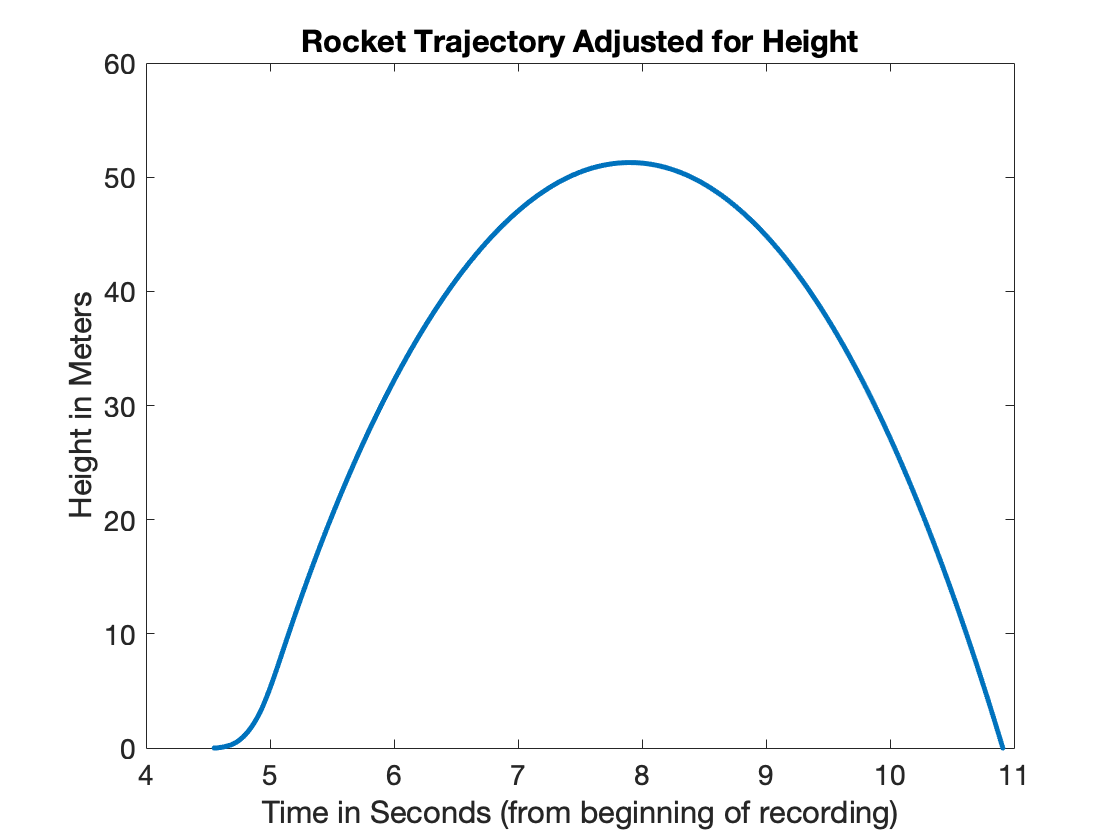
\includegraphics[width=\linewidth/3]{rockettraj.png}
    \end{center}
    \caption{Using acceleration minimum to adjust position}
    \label{fig:Rocket Trajectory}
\end{figure}
\begin{figure}[H]
    \begin{center}
    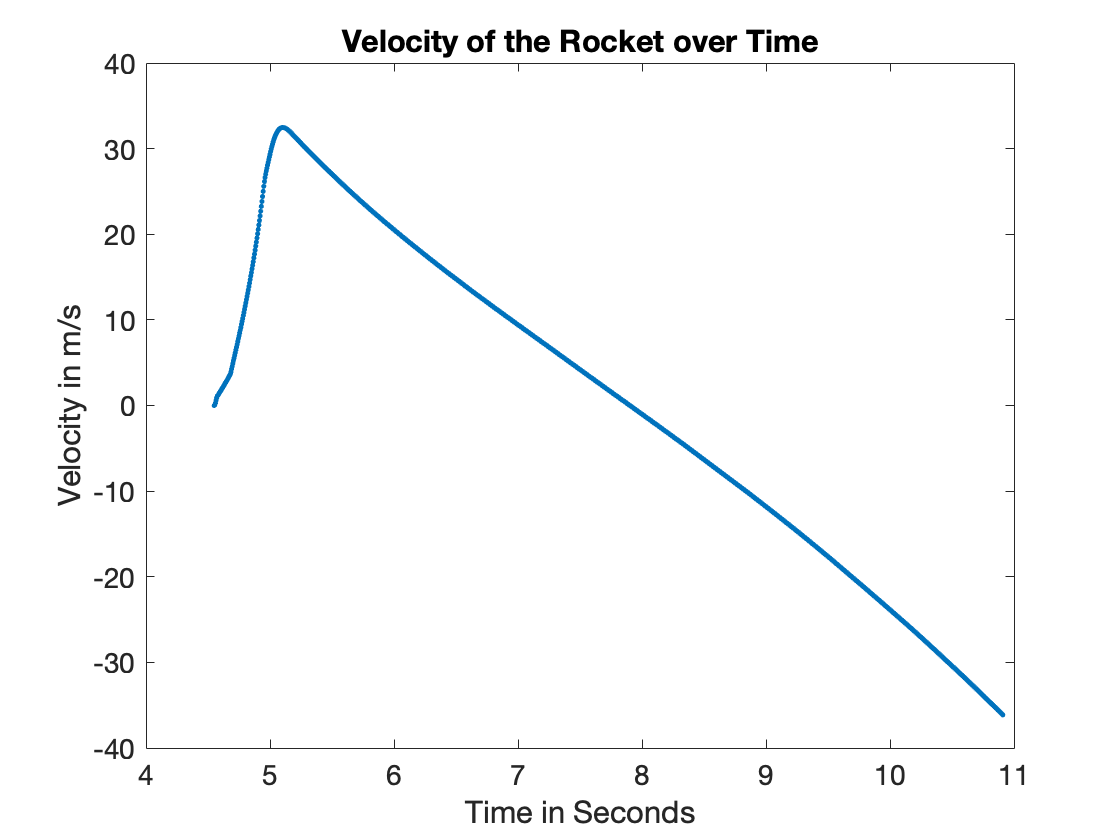
\includegraphics[width=\linewidth/3]{vel.png}
    \end{center}
    \caption{Graph of Velocity}
    \label{fig:Velocity}
\end{figure}
\begin{figure}[H]
\begin{center}
    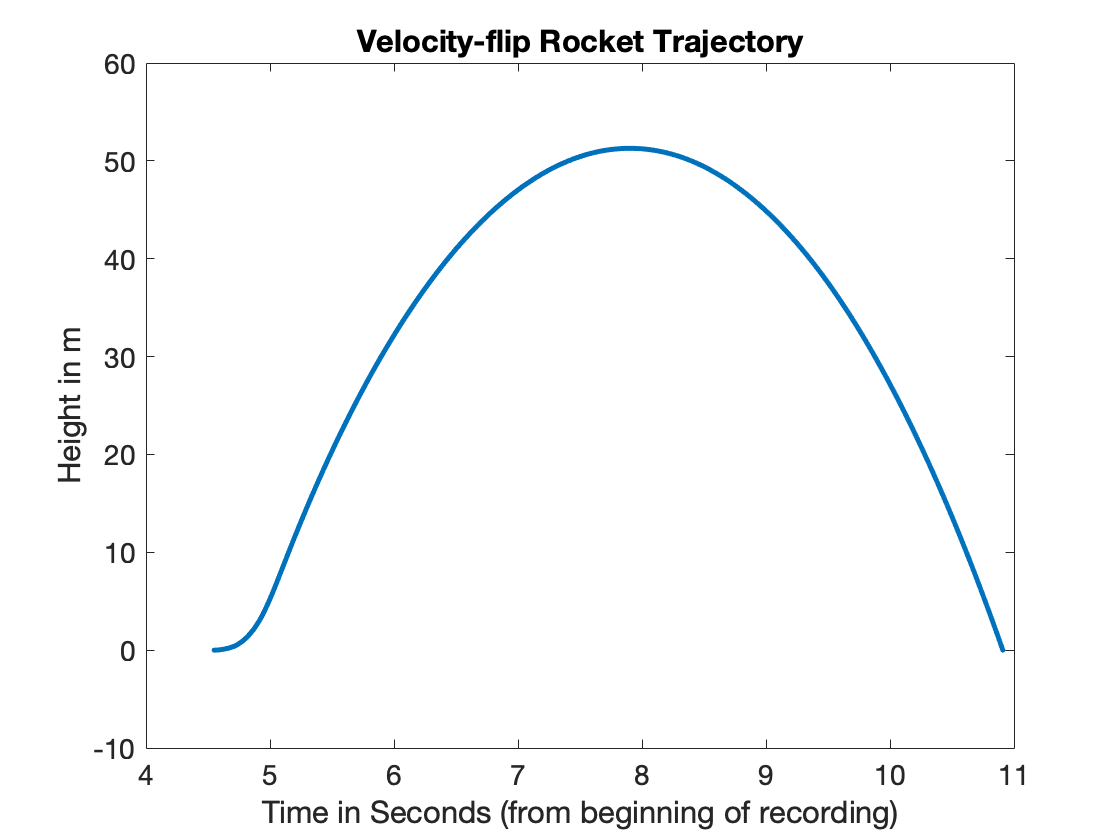
\includegraphics[width=\linewidth/3]{velrkttraj.png}
\end{center}
    \caption{Using Velocity sign-flip to adjust position}
    \label{fig:Rocket Trajectory}
\end{figure}

\section{Analysis Results}
{The launch index is $x$ = 910, the minimum acceleration occurs at $x$ = 1035, and the ground impact is $x$ = 2182. This corresponds to times 4.55 seconds, 5.175 seconds, and 10.91 seconds.}
{\quad I recalculated the callibration constant and offset using the upside down and right-side up data right after the launch, as well as each of the five flips on the table using the matlab script included below. For some reason, my calibration constants were drastically different from the rocket launch ones, but that may have been caused by the accelerometer failing to orient itself properly.}

\begin{equation} 
\textrm{S} = Ca + B
\end{equation}

\begin{figure}[H]
    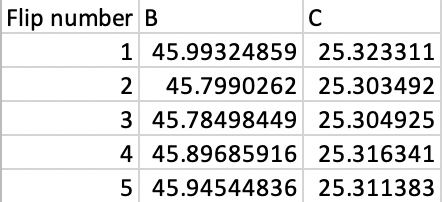
\includegraphics[width=\linewidth/4]{table.png}
\end{figure}

{From the B and C values taken, I took the mean and got 45.88 for $B$ and 25.31 for $C$. The constants after launch however were -13.02 and 25.16 ($B$ and $C$ respectively) so we can see that the $C$ constant drifts less for my accelerometer. I ended up using the B and C constants from launch in order to obtain a graph that made sense.}

{Using the the acceleration data as the derivative of the velocity, I found the point where it was closest to zero using the function $[m,i] = min(abs(v))$. The instant of velocity sign flip was thus 117 counts or .234 seconds after launch. }

{With the rocket flip included, the velocity is always positive, and suggests that the position of the rocket at landing is 427.4m. Using B and C from the launch, I obtained an angle of launch of $\frac{\pi}{13.554792}$ or approximately 13.28 degrees from the vertical when the landing point equaled zero.}
{My lab partners both had angles greater than mine, and ended up running further. I ran relatively a short distance–about 20-30m.}
\section{Conclusions}
{\quad This lab was spent analyzing the data we collected previously. This was important for understanding what the data meant as well as how to callibrate it. Ultimately we learned that the accelerometer drifts over time and if we do not callibrate for that drift, this drift can ultimately give incorrect data. }
\end{document}
